\section{Boundary condition one: visibility (on the anchor model)}
\label{sec:visibility}

% source: PAPER_SKELETON Sec 4; EVIDENCE_findings_core F-vis; reframed to Qwen-7B-scope per E1.

\paragraph{On Qwen2.5-7B, rejection is a step function of visibility.} When
the statement that would refute a planted falsehood is a directly readable
premise, at measured distance zero, the anchor model rejects the plant in
about 0.25 of continuations; one hop away the rejection rate collapses
roughly eightfold to 0.03, and it is flat for larger distances
(Figure~\ref{fig:visibility}).
% source: EVIDENCE_findings_core F-vis.1 (0.2467 d0 vs 0.0311 d1; flat 0.049/0.050/0.021)
Crucially, closure-valid completion is flat across distance, with a $d{=}0$
versus $d{=}1$ difference of $-0.002$ that is not significant, so the cliff
is a change in whether the model \emph{objects}, not a change in whether it
can finish the problem.
% source: EVIDENCE_findings_core F-vis.1 (closure diff -0.0024 p=0.893)
This contrast is measured directly but was left direction-open, so it
motivates the picture rather than clinching it.

\paragraph{The $d{=}0$ signal is pure premise read-out, not proof search.}
The abundant rejection at distance zero is entirely the model reading back a
contradiction that is already written in front of it. Within the licensed
split, which asks whether the model's own text contains a valid derivation,
all 111 of 111 $d{=}0$ rejections are premise read-out with zero written
derivations.
% source: EVIDENCE_findings_core F-vis.2 (111/111 d0_visible, 0 licensed)
This is why we call the effect visibility rather than checking: at $d{=}0$
the model sees the contradiction, it does not search for it.

\paragraph{Genuine multi-hop checking exists, but it is rare and not graded
by proximity.} We deliberately soften the strongest version of this claim.
It is not true that the model never performs even one hop of proof search:
the licensed split finds 235 complete written refuting derivations at
designed distance one or more, 95 of which require at least two real hops,
and among rejections whose complement is genuinely derivable the licensed
fraction is about 0.79.
% source: EVIDENCE_findings_core F-vis.2 (235 derivations, 95 >=2 hops, 0.789 licensed)
What is true is that this genuine checking is rare within any distance-one-
or-greater cell, a few percent, and it is not graded by proximity: the
licensed-derivation rate is flat across distance with no peak near the
plant.
% source: EVIDENCE_findings_core F-vis.2 (licensed 0.000/0.027/0.020/0.043/0.014, non-graded)
So the correct statement is that genuine distance-checking exists but is
rare and non-graded, and the large $d{=}0$ effect is visibility, not proof
search.

\paragraph{The one place genuine checking spikes is a cheap, useless hop.}
The exception is instructive. When a plant is inert, useless for the proof,
and its refutation is exactly one cheap hop away, the model does check: that
cell shows a rejection rate of about 0.19 that is 97 percent licensed
genuine one-hop checking, and the checking decays with distance to near
zero by three hops.
% source: EVIDENCE_findings_core F-vis.2 (cat_false_inert_d1 0.193, 96.6% licensed; 0.187->0.025->0)
This is a suggestive observation whose natural reading is that the model
checks when checking is cheap and the error is not useful to it. That reading
does not hold up: the usefulness of a planted statement does not detectably
change genuine checking. In a matched-pair construction that pits a useful
against a useless version of the same planted statement on matched worlds
(the question-flip experiment), the checking gap is null (gap $+0.004$, 95\%
CI $[-0.002, +0.010]$), and the earlier exploratory one-hop spike does not
replicate under this matched construction.
% source: E9_ADJUDICATION branch (b) NULL (primary gap +0.0037, CI95 [-0.00221,0.00958], excludes 0.164; inert-arm licensed ~0.011 vs E5 0.187); PROVISIONAL pending blind-rater audit
The forward-looking, causal version of this ``does the model's goal change
whether it checks'' question is a separate line of work
(Section~\ref{sec:related}), not a claim we make here.

\paragraph{A second, model-graded dependent variable reproduces the
cliff.} To rule out a regex artifact we re-scored all 11{,}577 rows with a
32B judge model. The judge reproduces the cliff, with judge-flagged doubt
about 0.13 at $d{=}0$ versus 0.03 at $d{=}1$, a factor of about four, then
flat, and it agrees with the lexical measure on 98 percent of rows.
% source: EVIDENCE_findings_core F-vis.3 (judge-doubt 0.127 d0 vs 0.029 d1; 98% agreement)
The judge's separate explicit-rejection measure carries a weak, gradual
tail beyond one hop, which is consistent with the rare non-graded checking
above rather than with a graded distance law; we report the doubt measure
as the clean cliff and note the tail.
% source: EVIDENCE_findings_core F-vis.3 caveat (rejection-DV tail 0.447/0.211/...)

\paragraph{The nearest rival account is addressability, and we stake the
claim where it is neutralized.} A concurrent account attributes such
effects to \emph{addressability}, the presence of a discrete referent to
act on, which coincides with visibility exactly at $d{=}0$
\citep{chen2026selfcorrection}. We concede the coincidence at $d{=}0$ and
therefore do not rest the claim there; we stake it on the flatness for
$d\ge1$, where a discrete refuting referent still exists in the world but
rejection has already collapsed.
% source: PAPER_SKELETON 4.6; RELATED_WORK_MAP P3 addressability

\paragraph{This visibility cliff is specific to Qwen2.5-7B.} Everything in
this section is measured on the anchor model, and the multi-model
replication of Section~\ref{sec:usability} shows the cliff does not
generalize: on three of four further models the $d{=}0$ contrast
significantly reverses. We keep the visibility law scoped to Qwen2.5-7B and
treat the reversal itself as a finding.
% source: E1_ADJUDICATION Sec 3 B1; F-vis.1 E1 caveat

\begin{figure}[t]
\centering
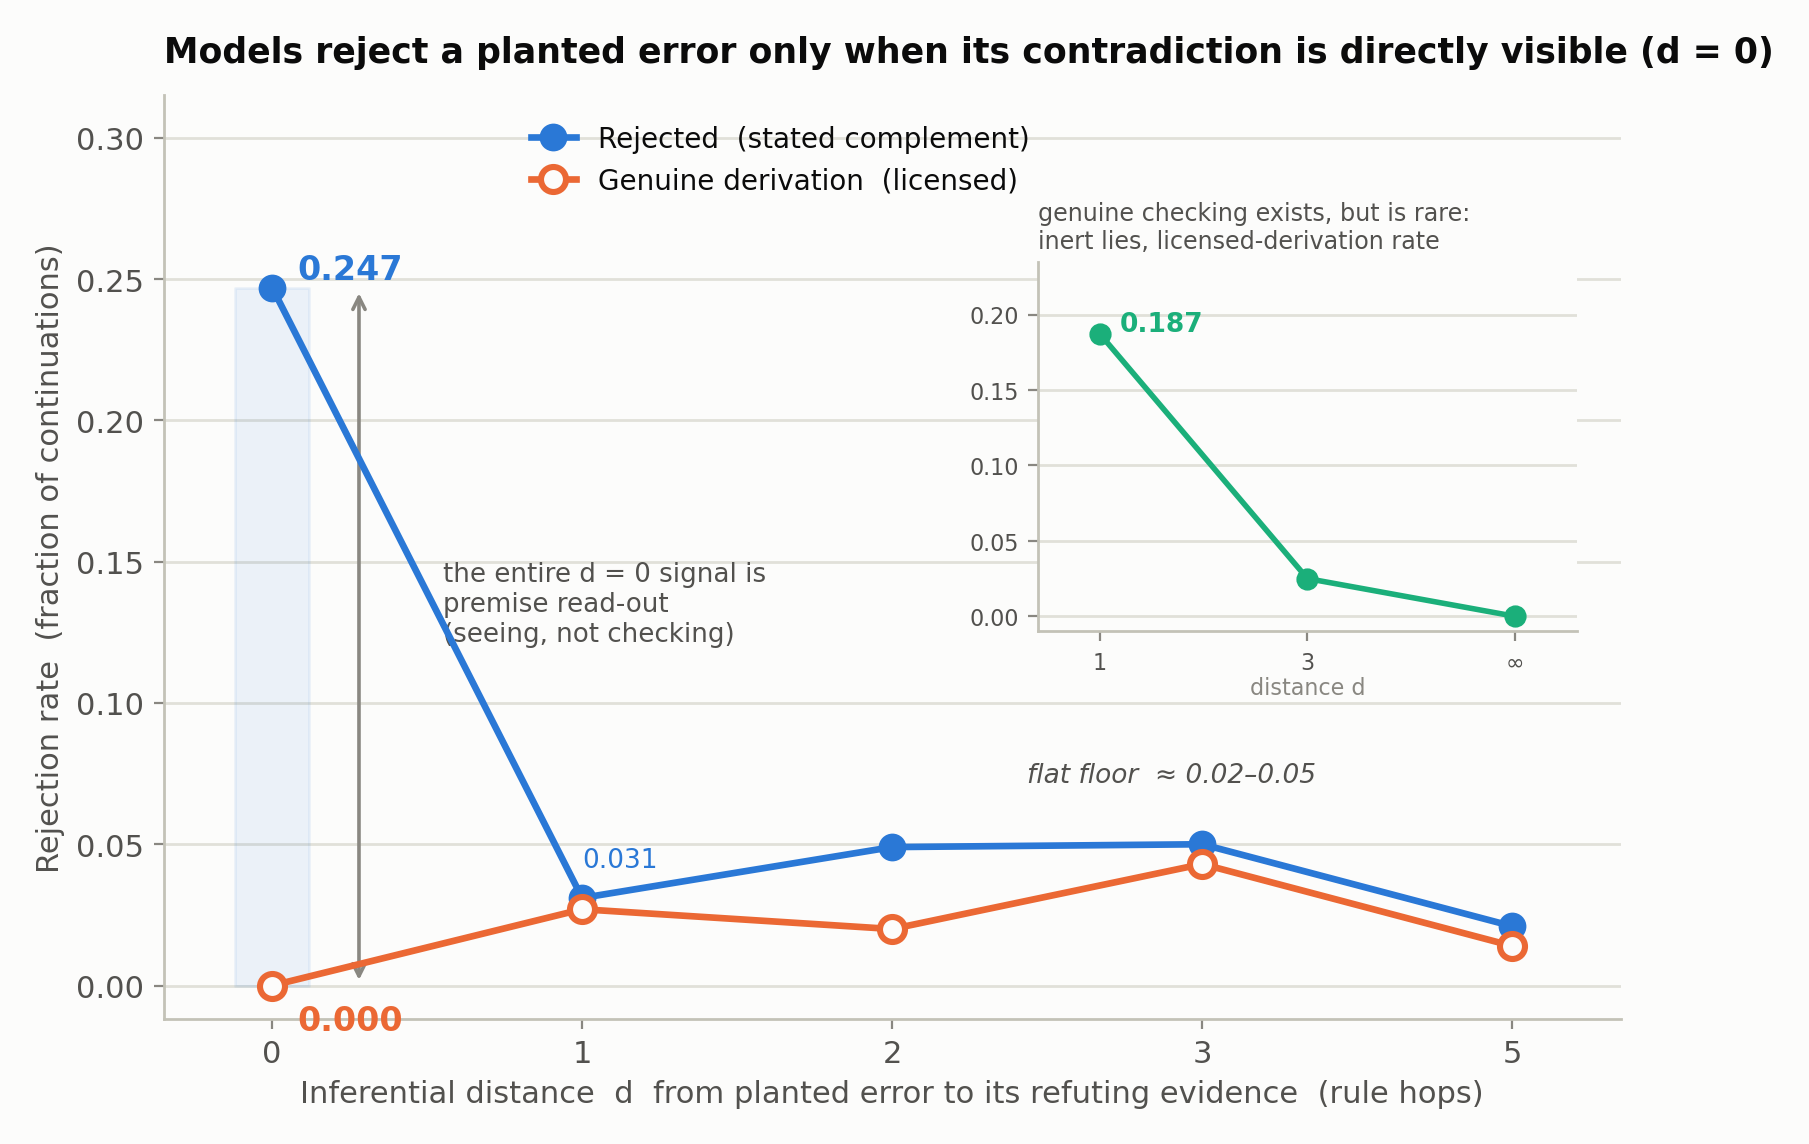
\includegraphics[width=0.82\textwidth]{figures/fig_b_visibility_cliff.png}
\caption{\textbf{The visibility cliff on Qwen2.5-7B, and why it is
``seeing'' not ``checking''.} Explicit rejection (stated complement) of a
planted falsehood peaks at measured distance $d{=}0$ (0.25) and collapses to
a flat floor for $d\ge1$ (0.03 at $d{=}1$). The licensed-only overlay,
rejections backed by a genuine written derivation, is \emph{zero} at
$d{=}0$: the entire $d{=}0$ signal is premise read-out. Genuine multi-hop
checking is not absent (235 written derivations exist at $d\ge1$, 95 needing
two or more hops) but it is rare and not graded by proximity. The inset
shows the one real distance-check, the inert one-hop cell (0.19 rejection,
97\% licensed), decaying with distance. \emph{This figure is Qwen2.5-7B
only}; \todo{add a per-model strip from the multi-model replication showing
the cliff reverses on Llama-3.1-8B / Qwen2.5-1.5B / Qwen2.5-32B.} Licensed
numbers are the strict v2 classifier.}
% source: figures/FIGURE_CAPTION_PLANS Fig B
\label{fig:visibility}
\end{figure}
